% !TEX root = ../../main.tex

\subsection{Impact of framework structure on transition mechanics}%
\label{dut:comparison}

While the discovery of the NGA transition in DUT-49 was a result 
of serendipity, it opens the door to a rational design approach 
to modify the extent and the location of the phenomenon. In principle,
there are several avenues that could be taken in order to tune the 
contraction mechanics.
\begin{itemize}
    \item Changing the range of metastability of the open pore state.
    \item Decreasing the porosity of the closed pore state.
    \item Increasing the capacity of the open pore form.
\end{itemize}
These factors are bound to be tightly interlinked, with a slight 
alteration in one possibly leading a shift in all. For example, the 
addition of a stabilizing group which would increase the tensile 
strength of the linker is also likely to decrease the porosity 
of the entire system.

There are a range of physicochemical modifications available to 
tune the properties of the framework, many already employed in the
MIL-53 and MIL-47 family of flexible MOFs.
Through functionalisation or modification of the linker, the strength of the guest-guest
and guest-host interactions is affected, as evidenced by the different
gate opening behaviour with nitrogen and water on several functionalised
versions on MIL-53~\cite{biswasNewFunctionalizedFlexible2011}.
In the case of DUT-49, moieties grafted to the central strut or changes
in the linker backbone are also likely to affect its buckling behaviour.
The use of a different metal as the node, has succeeded in changing the 
mechanical response of MIL-53~\cite{yotImpactMetalCentre2016}. This 
approach is likely have less impact on DUT-49, as the mechanism of 
contraction is due to linker flexibility.
A common rational design methodology is the so-called isoreticular design,
where topologically isomorphic MOFs are synthesised through progressive elongation
of the linker. Another path to controlling flexibility is manipulation of crystal 
size, as it has already been shown by \citet{krauseEffectCrystalliteSize2018}.
Finally, structural defects, of which a description was given 
in \autoref{def}, are another degree of freedom to consider for NGA 
tunability. Approaches such as mixed linkers synthesis and vacancy defects
may allow for fine-grain influence of framework stiffness.

\subsubsection{Behaviour of isoreticular materials}

The series of materials DUT-48, DUT-46, DUT-49, DUT-50 and DUT-151/DUT-152
was synthesised with the aim of studying the effect of linker 
elongation on the NGA step. It was found that the tetra-phenyl chain
in DUT-151 increased the pore size to the threshold 
where a secondary can form in the intracrystal voids, resulting 
in two identical interpenetrated nets. An attempt to introduce 
a bulky side-functionalisation in DUT-152 resulted in a similarly
interpenetrated material. \autoref{dut:fgr:dut-reticular} shows the
butane adsorption dataset recorded on the non-interpenetrated versions.

\begin{figure}[htb]
    \centering
    \begin{subfigure}{0.33\linewidth}
        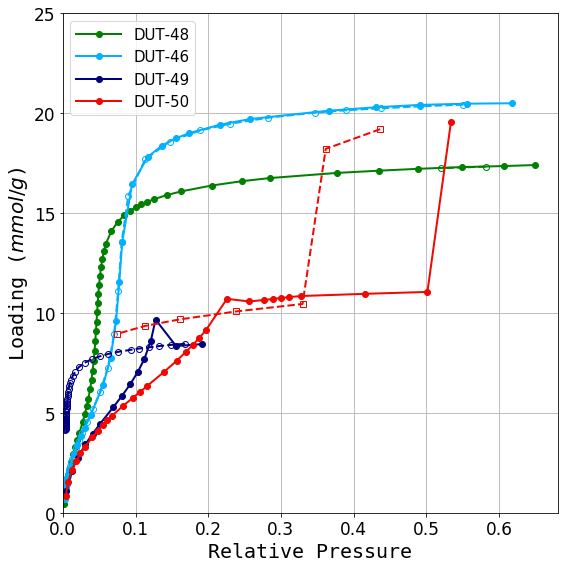
\includegraphics[width=\linewidth]{rtc/dut-reticular-reg}%
        \caption{}\label{dut:fgr:dut-reticular-reg}
    \end{subfigure}%
    \begin{subfigure}{0.33\linewidth}
        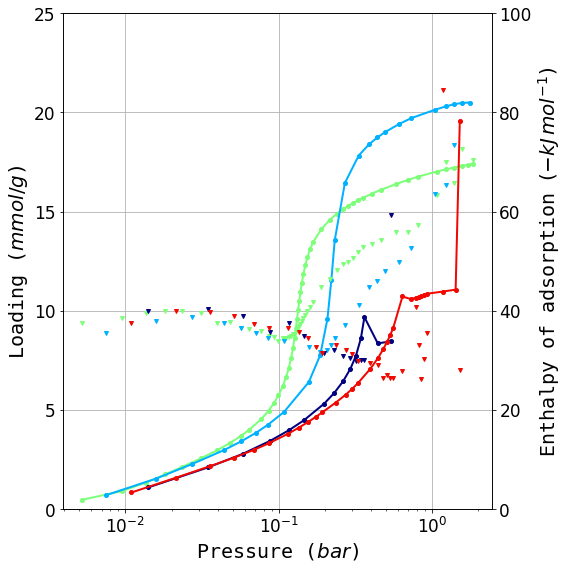
\includegraphics[width=\linewidth]{rtc/dut-reticular-log}%
        \caption{}\label{dut:fgr:dut-reticular-log}
    \end{subfigure}%
    \begin{subfigure}{0.33\linewidth}
        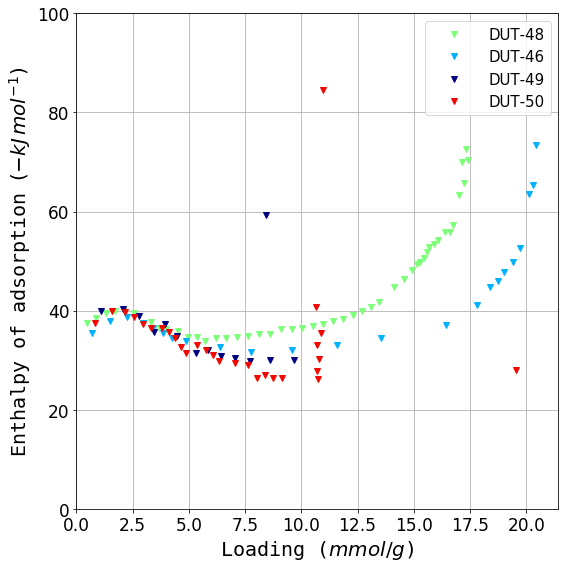
\includegraphics[width=\linewidth]{rtc/dut-reticular-enth}%
        \caption{}\label{dut:fgr:dut-reticular-enth}
    \end{subfigure}%
    \caption{(a) Experimental adsorption isotherms for DUT-48, DUT-46, DUT-49 and 
    DUT-50. Enthalpy points are omitted for clarity. (b) A logarithmic plot of 
    isotherms and enthalpy curves, to highlight the low pressure region. 
    (c) Differential enthalpy of adsorption as a function of loading.}%
    \label{dut:fgr:dut-reticular}
\end{figure}


Indeed, the results follow a predictable trend. First, it is worth 
noting that, as seen in \autoref{dut:fgr:dut-reticular-reg}, only DUT-49 
and DUT-50 undergo an \textbf{op/cp} transition. This confirms that 
a shorter linker imparts the resulting MOF with a more stable backbone,
raising the strain required in order to collapse the framework.
The desorption branch of the non-flexible materials completely 
overlaps the adsorption branch in both isotherm and enthalpy, further
confirming the small error in measurement (available in 
\autoref{appx:dut:fgr:dut-46-adsdes}).
With an increase of linker size, a larger pore volume and consequently
a higher amount of butane can be adsorbed in the open pore form. 
The increase in pore size is also responsible for a shift in the pressure 
of condensation, or pore filling step.

In DUT-50, the structure is seen to re-open around \(0.5~p/p_0\), although 
the pressure is not high enough to completely transition to the
\textbf{op} form. The collapse to the closed phase in the desorption
branch achieves a lower plateau than in the adsorption branch,
suggesting an incomplete \textbf{op/cp} transition as seen in one 
of the isotherms on DUT-49 in the previous section.

One surprising finding is that the enthalpy curves 
(\autoref{dut:fgr:dut-reticular-enth}) present a near
identical behaviour and differential enthalpy of adsorption in the 
low pressure region, characterized by a slight increase up to 
\SI{40}{\kilo\joule\per\mol} followed by a drop-off. The adsorption
mechanism and surface characteristics are therefore \textit{common} to 
all four materials. The shift of the enthalpies of adsorption to lower 
values at higher loadings from DUT-46 to 50 is expected, with the increase
in pore size leading to a progressive decrease of the contribution 
of dispersion interactions with the guest, which could also be 
referred to as a confinement effect. The the steep uptake in the isotherm
is indicative of a cooperative adsorption mechanism similar to a fluid
condensation, accompanied by an increase in the contribution of 
guest-guest interactions to \(\Delta_{ads} \dot{h}\).

As neither DUT-48 and DUT-46 show any phase transition with
butane at this temperature, the question arises whether their frameworks
can still undergo a structural contraction. A combined simulation and 
mechanical pressure study was performed on DUT-48 in parallel to the 
microcalorimetry experiments, which can be found in the paper 
published in collaboration with the TU Dresden, Chimie ParisTech and 
ICGM groups~\cite{krauseAdsorptionContractionMechanics2018}.
In brief, DFT optimisations of a single linker molecule under increasing
stress show that buckling of the molecule is still possible, albeit
at a much higher stress. Constant volume (N, V, T) molecular dynamics
simulations of the evolution of the system free energy with decreasing
unit cell volume have shown that, while a \textbf{cp} phase for DUT-48
exists, the increased tensile strength of the central backbone leads
to an increase in both the free energy of this state and the activation
energy required to enter it compared to DUT-49. To prove that structural
transition can still take place, mercury intrusion experiments are 
carried out on both DUT-48 and DUT-49. The intrusion/extrusion 
curves on both materials show that an \textbf{op/cp} transition takes
place, although with a much higher external pressure in the case 
of DUT-48 (\SI{65}{\mega\pascal} vs.\ \SI{35}{\mega\pascal}). A similar 
approach on all other materials in this series reveals a very clear
trend in both energy of the \textbf{cp} form and pressure required 
for the transition.

\begin{figure}[htb]
    \centering
    \begin{subfigure}{0.5\linewidth}
        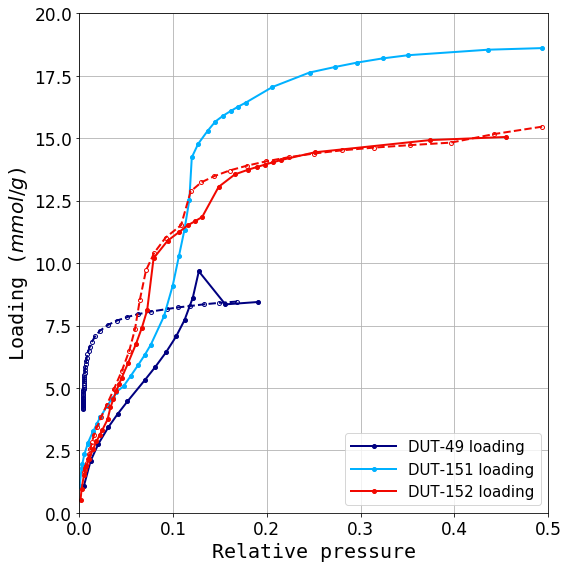
\includegraphics[width=\linewidth]{rtc/dut-reticular-interp-reg}%
        \caption{}\label{dut:fgr:dut-reticular-interp-reg}
    \end{subfigure}%
    \begin{subfigure}{0.5\linewidth}
        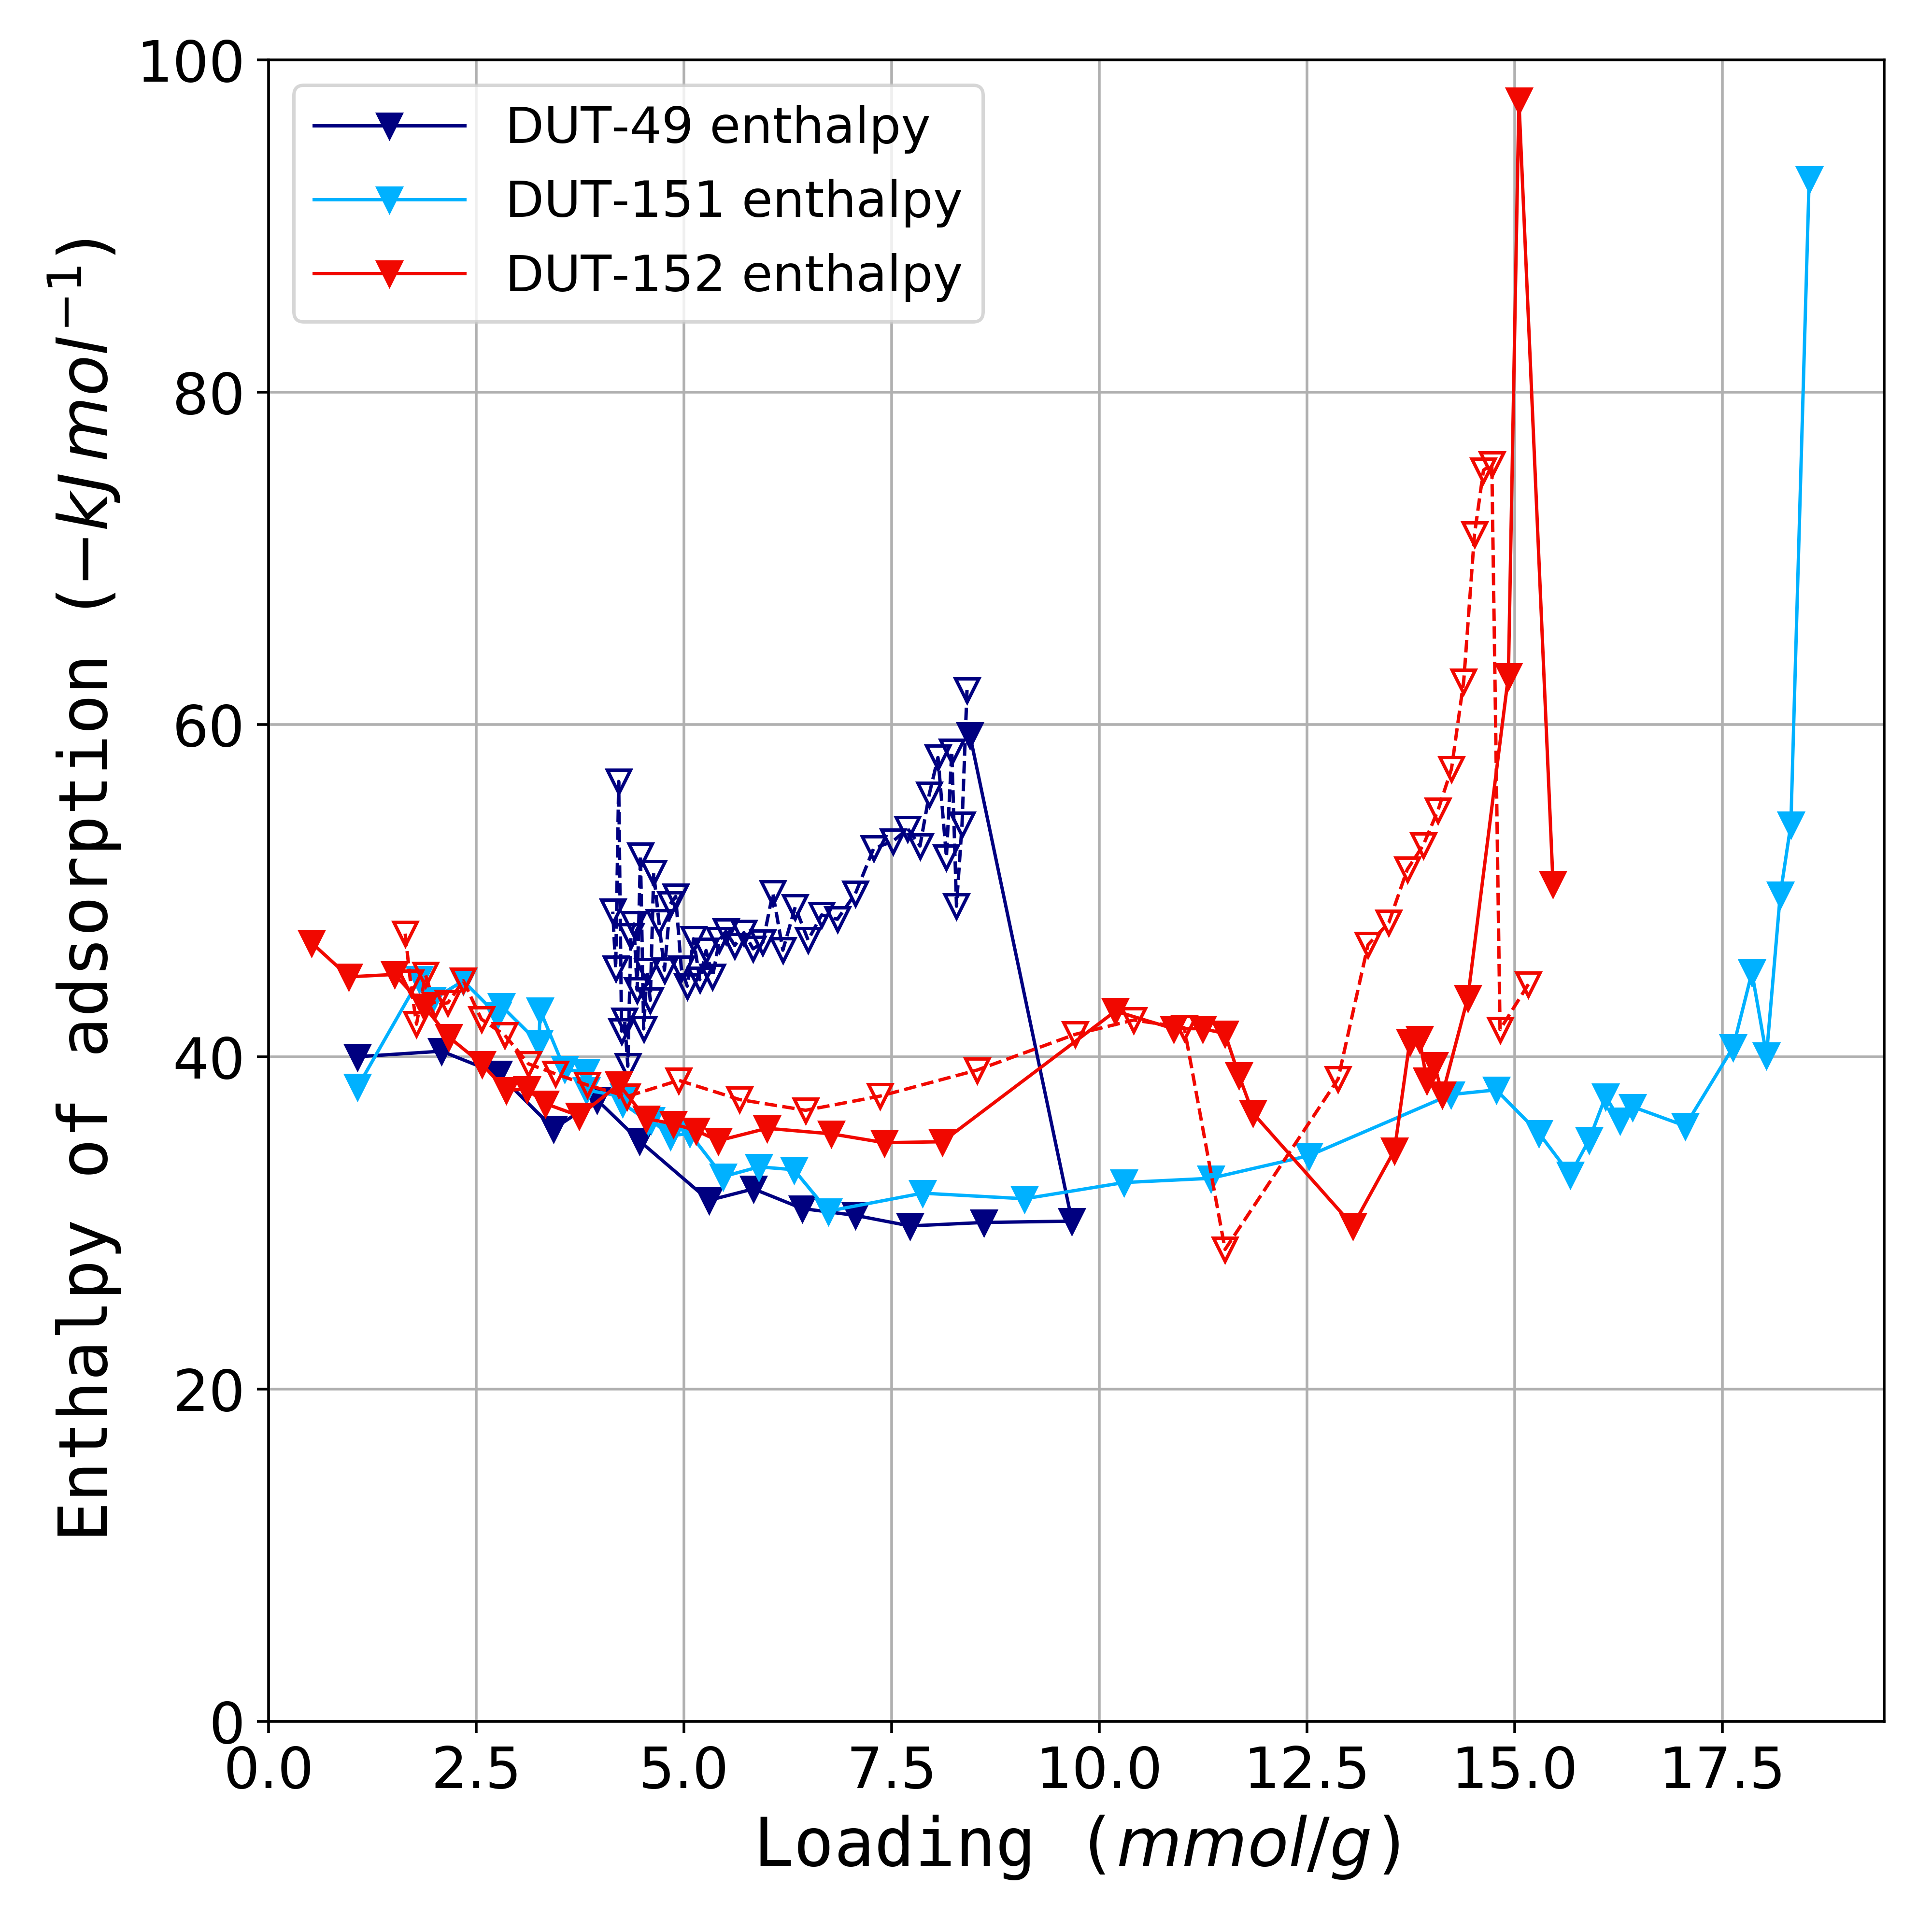
\includegraphics[width=\linewidth]{rtc/dut-reticular-interp-enth}%
        \caption{}\label{dut:fgr:dut-reticular-interp-enth}
    \end{subfigure}%
    \caption{The (a) isotherms and (b) enthalpy curves of the
    interpenetrated materials DUT-151 and DUT-152 as compared to 
    DUT-49. Shaded regions are guides for the eye rather than
    uncertainty domains.}%
    \label{dut:fgr:dut-reticular-interp}
\end{figure}

The interpenetrated materials DUT-151 and DUT-152 show a very different 
isotherm shape and enthalpy curve, as presented in 
\autoref{dut:fgr:dut-reticular-interp}. In their case, the adsorption
behaviour is very complex, with multiple transitions and 
hysteresis loops visible. However, several trends can still be rationalized.
The total pore volume of DUT-152 is lower than that of DUT-151, as 
the bulkier central strut lowers the available space. Both materials 
show steeper adsorption curve at low pressures, due to the increased 
interactions of the adsorbate molecules with the doubled framework
net. This is reflected in the differential adsorption enthalpy 
in the same region, with both DUT-151 and 152 displaying a higher
enthalpy (\SIrange{45}{50}{\kilo\joule\per\mol} as opposed to 
\SI{40}{\kilo\joule\per\mol} for DUT-49). The smaller pore size 
of DUT-152 also leads to a shift in the adsorption isotherm to
lower pressures and an increased enthalpy of adsorption at higher 
loadings. Finally, a total of three hysteresis loops are visible 
on DUT-152 associated with apparent transitions, highlighting several
accessible intermediate pore states in its structure. These transitions
are also found in the enthalpy curve, a result of different energetic
contributions of the contraction/expansion. In order to elucidate 
such a complex interplay of factors more powerful methods such
as \textit{in-situ} PXRD are required to monitor the change of
structural parameters during adsorption. While interesting,
it should be pointed out that all transitions on DUT-151 and 152 
seem to be continuous phase changes, with no potential for an
NGA-type contraction.

\subsubsection{Behaviour of ``reinforced'' linker analogues}

A series of DUT-49 analogues, DUT-149, DUT-148 and DUT-147, 
with progressively connected central additions was created in
order to observe the effect of linker strengthening on the 
structural transition. DUT-149 has two methyl groups in the 
ortho position relative to the central bond. DUT-148 has 
the same carbon number, but connects the two methyl groups
with a single bond. Finally DUT-147 has a fully aromatic
structure, with delocalised double bonds on each side of the 
original phenyl ring. The resulting isotherm and enthalpy 
curve are shown in \autoref{dut:fgr:dut-func}.

\begin{figure}[htb]
    \centering
    \begin{subfigure}{0.33\linewidth}
        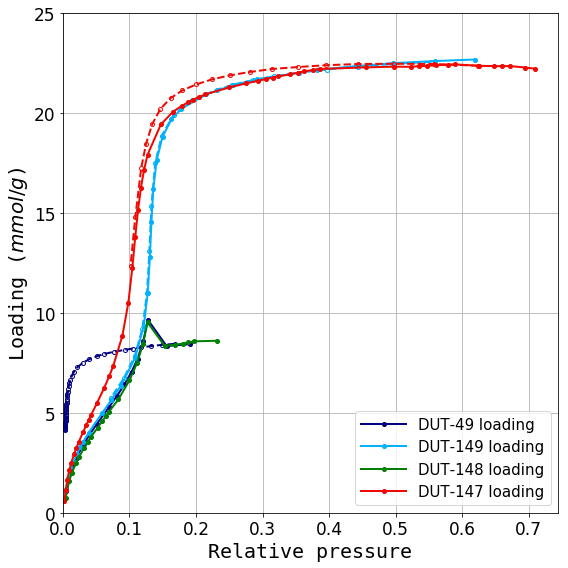
\includegraphics[width=\linewidth]{rtc/dut-func-reg}%
        \caption{}\label{dut:fgr:dut-func-reg}
    \end{subfigure}%
    \begin{subfigure}{0.33\linewidth}
        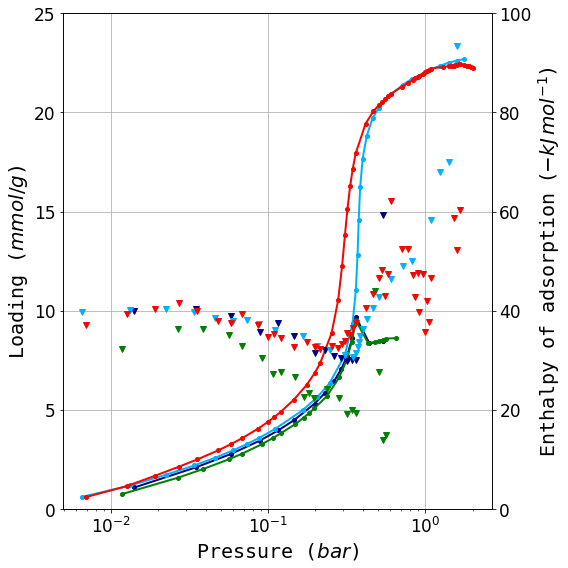
\includegraphics[width=\linewidth]{rtc/dut-func-log}%
        \caption{}\label{dut:fgr:dut-func-log}
    \end{subfigure}%
    \begin{subfigure}{0.33\linewidth}
        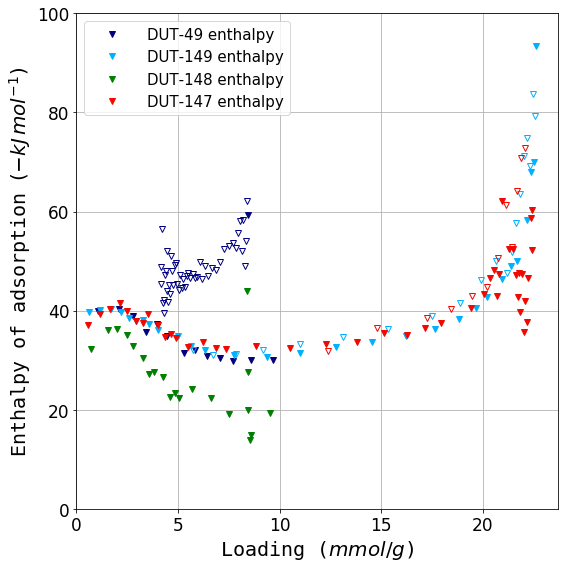
\includegraphics[width=\linewidth]{rtc/dut-func-enth}%
        \caption{}\label{dut:fgr:dut-func-enth}
    \end{subfigure}%
    \caption{(a) Experimental adsorption isotherms for DUT-49, DUT-149,
    DUT-148 and DUT-147. Enthalpy points are omitted for clarity. 
    (b) A logarithmic plot of isotherms and enthalpy curves,
    to highlight the low pressure region. 
    (c) Differential enthalpy of adsorption as a function of loading.}%
    \label{dut:fgr:dut-func}
\end{figure}

An unexpected trend emerges from the measured isotherms. DUT-149
does not show an NGA step, with adsorption taking place entirely
on the \textbf{op} form of the material. In this regard it is
an almost perfect non-flexible variant of DUT-49, with near-complete
overlap of both its isotherm and enthalpy curves. A minute 
shift to lower pressure can be seen in the isotherm, as the 
methyl groups introduce a slight decrease in the large octahedral
and medium tetrahedral pore size. Counterintuitively, the next material
in the series, DUT-148, undergoes structural contraction in the
same manner as DUT-49, retaining the NGA transition despite its 
increased connectivity. Finally, DUT-147 is stiffer and maintains
its \textbf{op} state throughout adsorption. A wide hysteresis
appears in the desorption branch, which may be an indication of 
subtle structural effects such as a rotation of the central part
of the linker.

\begin{figure}[htb]
    \centering
    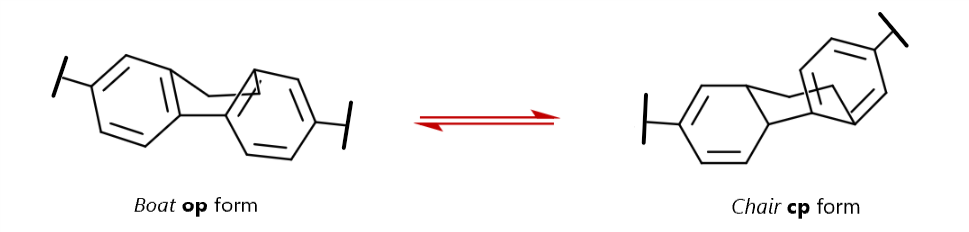
\includegraphics[width=0.8\linewidth]{structures/DUT-148-flip}%
    \caption{A possible mechanism for a conformer stabilised 
    \textbf{op/cp} transition for DUT-148.}%
    \label{dut:fgr:dut-148-flip}
\end{figure}

The different behaviour these analogues may have two possible
causes: a change in the stability of the \textbf{cp} phase or a 
difference in the stain necessary to induce ligand buckling. Both
parameters are influenced by the introduced functionalisations. 
In the case of DUT-147 the central phenyl-phenyl bond
has been strengthened, resulting in an increased strain required to
induce the transition. For DUT-148 and DUT-149 the source of the 
counterintuitive trend is less clear-cut. In DUT-149, the methyl
groups are sterically hindered, which results in the likely
adoption of the lowest energy state, with the two phenyl rings
at a \ang{180} angle with each other and \ang{90} degree with the
terminal ligand planes. 
This steric hindrance may increase the required strain to 
enter the elastic buckling regime. Conversely, the 
single bond in DUT-148 restricts the alkyl chain to a single 
side of the bond and may actually lower the energetic barrier for
the existence of the \textbf{cp} form, through the stabilisation
afforded by a chair-like 6-ring conformer, a possible variant 
of which can be seen in \autoref{dut:fgr:dut-148-flip}. 
DFT optimisations, as 
those performed on the previous isoreticular linkers are 
recommended to shed light on the buckling behaviour.

\subsubsection{Behaviour of heterocyclic DUT-49 analogues}

Using a thiophene-substituted aromatic linker may introduce additional
guest-host interactions due to the resulting heterogeneous pore
surface. Additionally, the change in geometry allows for new 
flexibility modes. The butane isotherms measured on these materials
are summarized in \autoref{dut:fgr:dut-heterocyc}.

\begin{figure}[htb]
    \centering
    \begin{subfigure}{0.33\linewidth}
        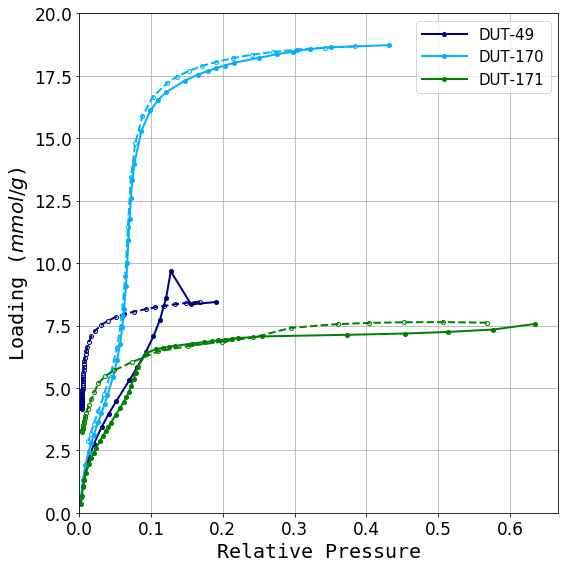
\includegraphics[width=\linewidth]{rtc/dut-heterocyc-reg}%
        \caption{}\label{dut:fgr:dut-heterocyc-reg}
    \end{subfigure}%
    \begin{subfigure}{0.33\linewidth}
        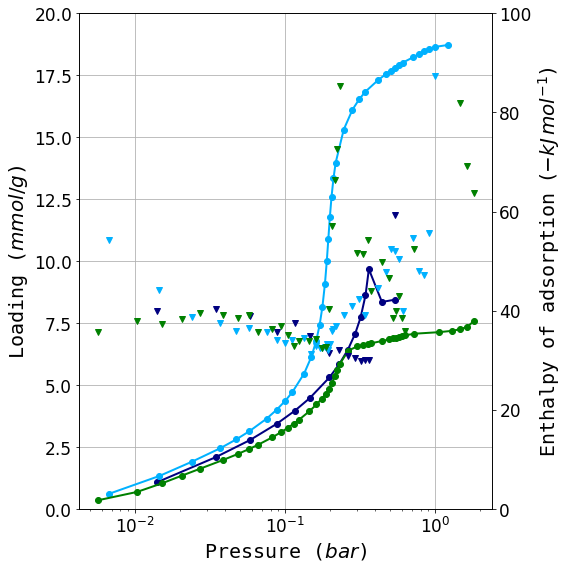
\includegraphics[width=\linewidth]{rtc/dut-heterocyc-log}%
        \caption{}\label{dut:fgr:dut-heterocyc-log}
    \end{subfigure}%
    \begin{subfigure}{0.33\linewidth}
        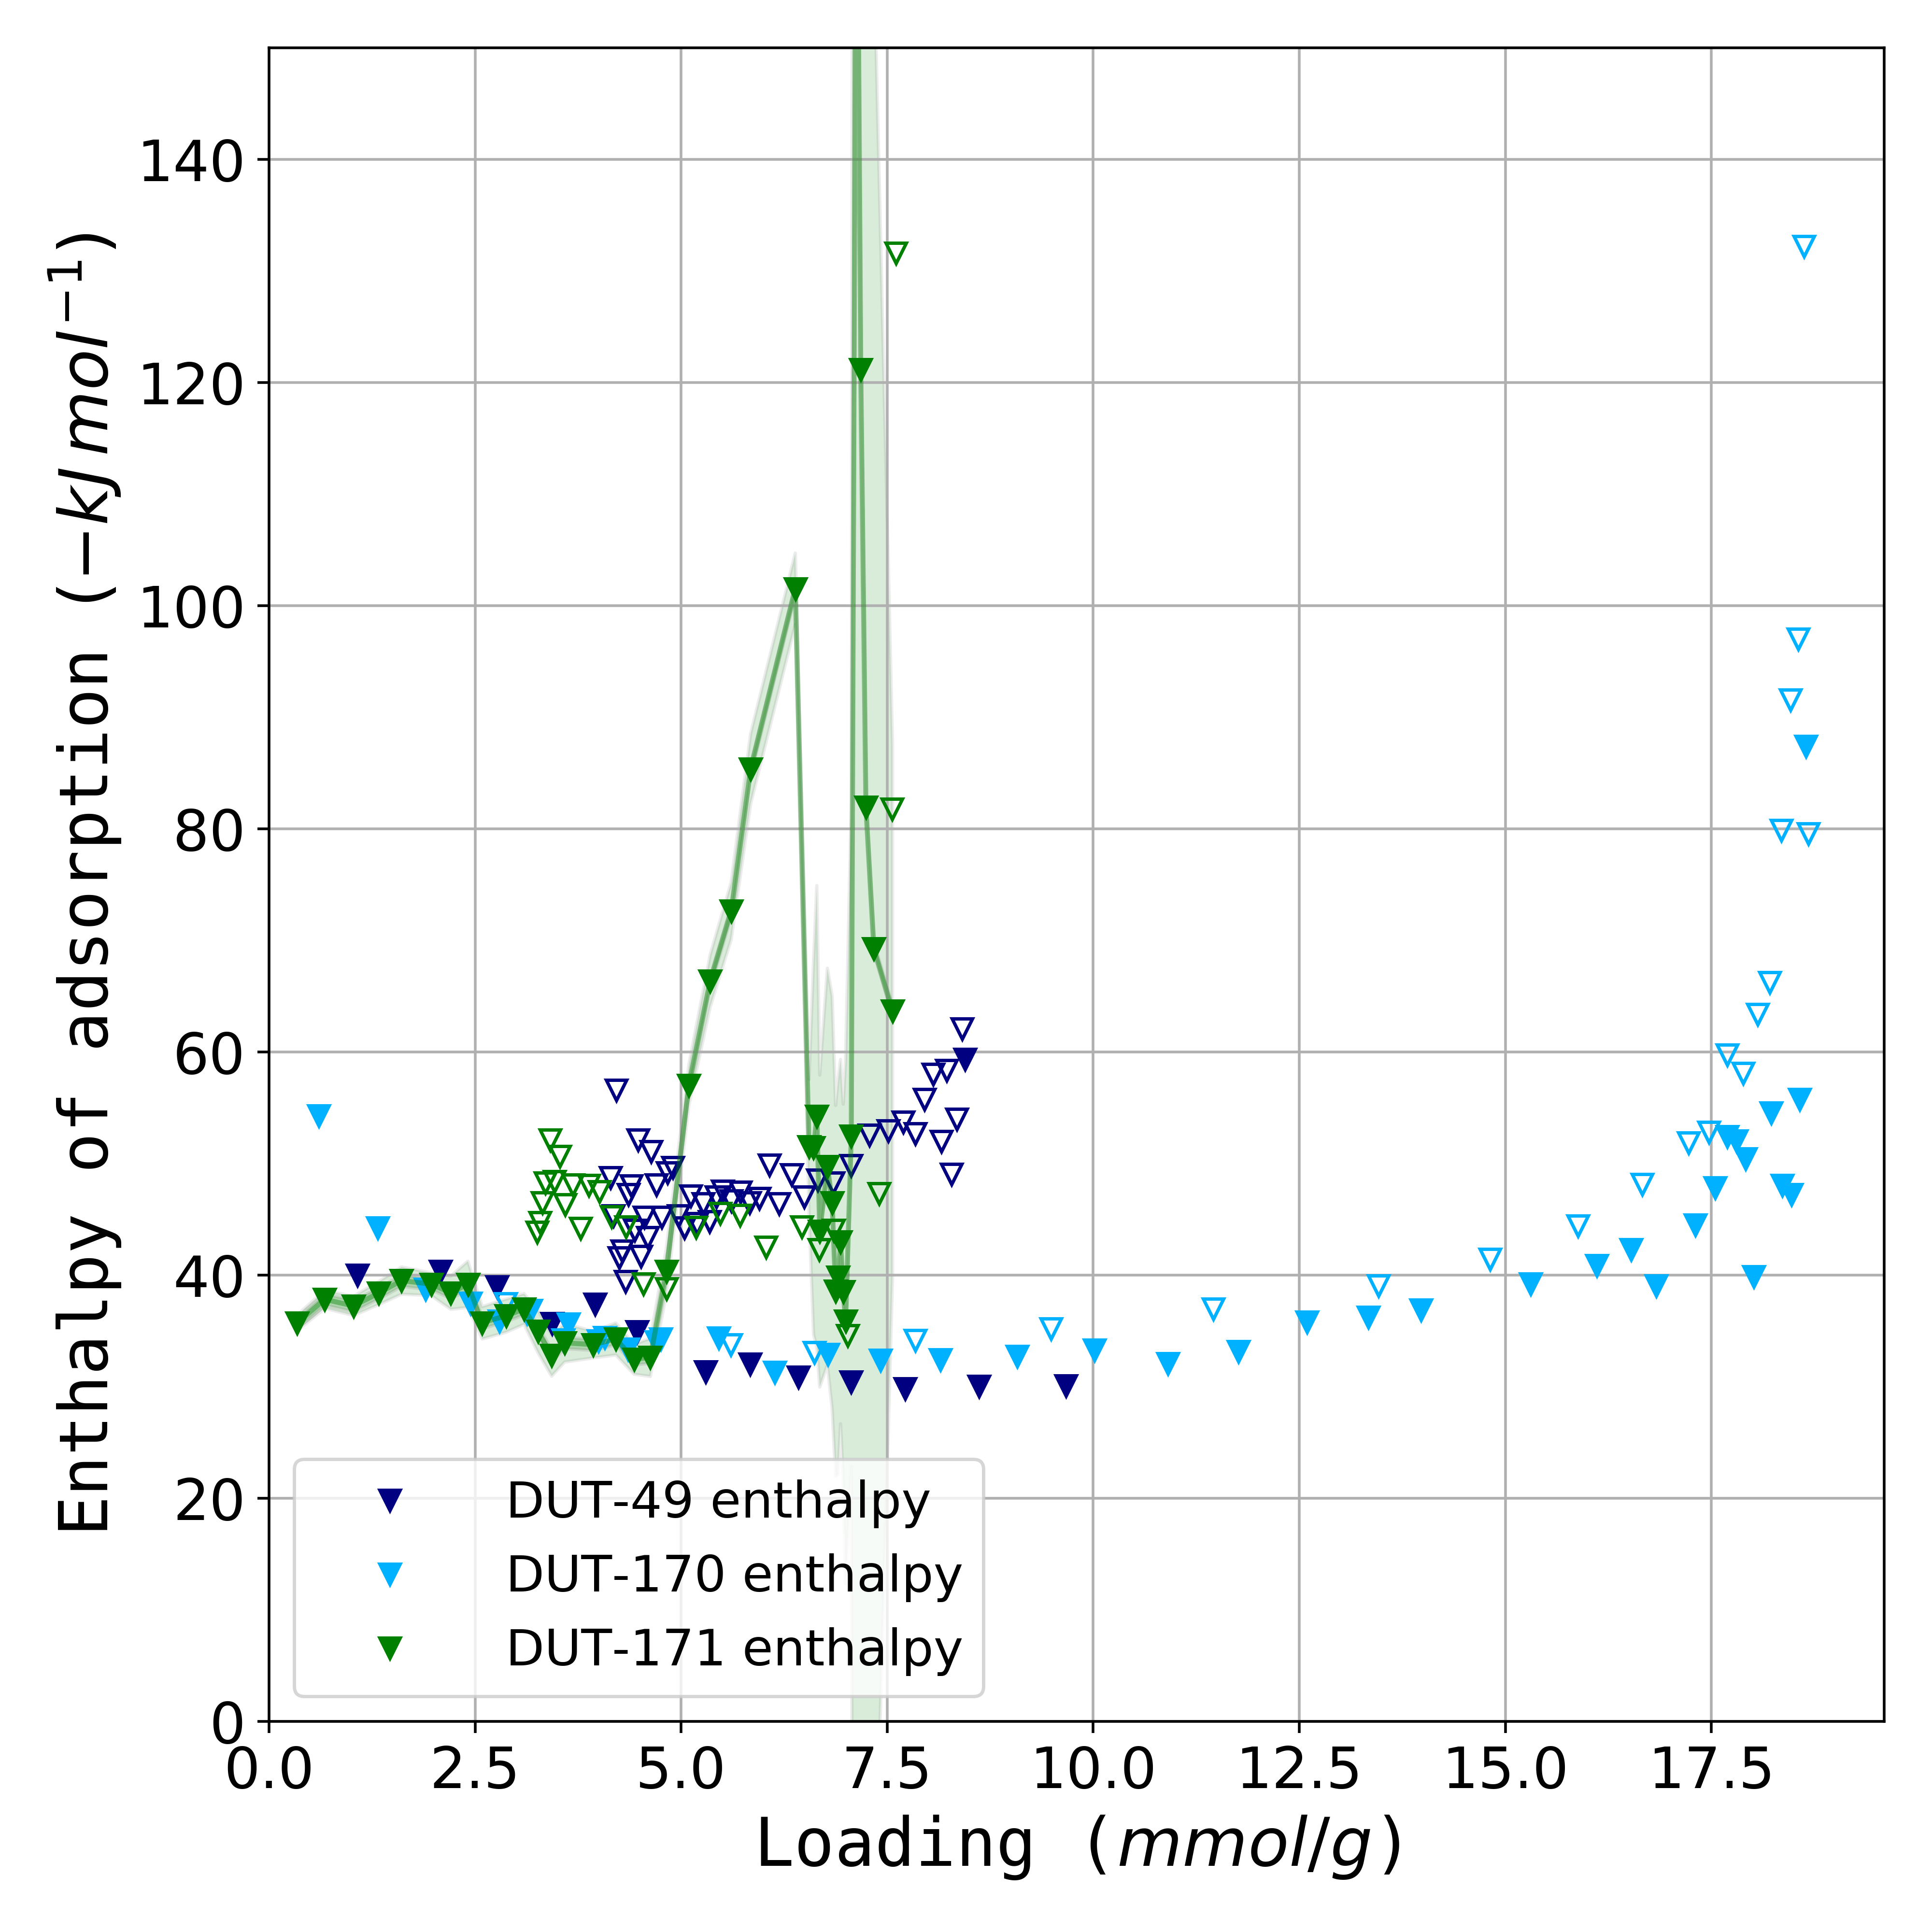
\includegraphics[width=\linewidth]{rtc/dut-heterocyc-enth}%
        \caption{}\label{dut:fgr:dut-heterocyc-enth}
    \end{subfigure}%
    \caption{(a) Experimental adsorption isotherms for DUT-49 and 
    heterocyclic analogues DUT-170 and DUT-171. 
    Enthalpy points are omitted for clarity. 
    (b) A logarithmic plot of isotherms and enthalpy curves
    to highlight the low pressure region. 
    (c) Differential enthalpy of adsorption as a function of loading, highlighting the 
    adsorption branch and error range of DUT-171.}%
    \label{dut:fgr:dut-heterocyc}
\end{figure}

DUT-170, which has a linker with a similar structure and length as
the naphtyl-derived DUT-48 is expected to remain non-flexible.
This is seen to be the case, with the two isotherms similar in 
regard to total amount adsorbed and pore filling pressure. 
The isotherm of DUT-171 does show a structural transition, 
but without any observed NGA. A slight hysteresis can be seen,
likely due to partial structure re-opening before the beginning 
of the desorption branch. Instead of NGA, the enthalpy curve 
reveals a significant departure from the baseline as the 
slope of the isotherm changes slowly in a manner indicative
of continuous contraction to a \textbf{cp} form. The resulting phase 
has enthalpies of desorption in the same range as DUT-49\textbf{cp}.
This type of continuous phase change may suggest a different 
ligand deformation mechanism, without a sudden buckling and 
more akin to an elastic bending regime, perhaps due to the 
starting zig-zag shape of the linker.

Finally, the low pressure region of the enthalpy curve for 
DUT-170 shows a a higher differential enthalpy of adsorption.
However, a repeat of the experiment found that instead of 
a specific interaction of the heterocycle with the guest,
this anomaly is due to poor thermal equilibration of the 
sample cell before the start of data recording in that 
particular measurement.

\subsubsection{Behaviour of elongated central strut materials}

The final series of synthesised materials comprise DUT-160, 
161 and 162, materials with a triple, double and single bond 
inserted between the central phenyl rings. Unfortunately, 
DUT-162 cannot be obtained in a desolvated open pore form, as it 
immediately collapses upon supercritical activation. Furthermore,
the yield of DUT-160 and 161 was so low that not enough 
material was available for an experiment with DUT-161, and resulted
in larger errors in the enthalpy curve of DUT-160. In particular 
the behaviour of DUT-161 could prove interesting, as the linker 
may exist in either a \textit{trans} or \textit{cis} isomer.
The recorded isotherms are presented in \autoref{dut:fgr:dut-sat}.

\begin{figure}[htb]
    \centering
    \begin{subfigure}{0.33\linewidth}
        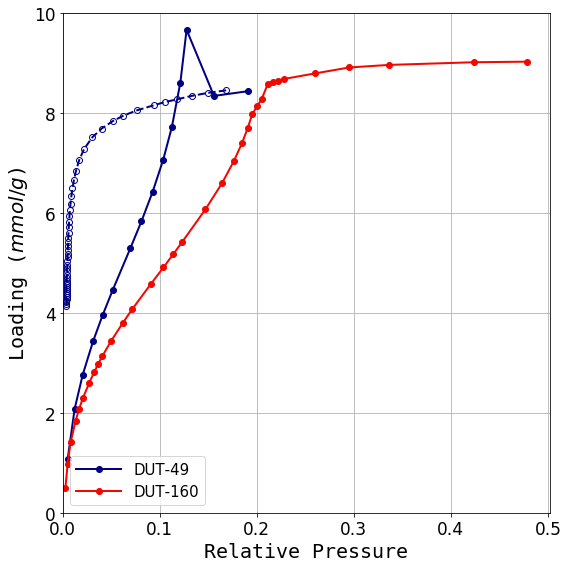
\includegraphics[width=\linewidth]{rtc/dut-sat-reg}%
        \caption{}\label{dut:fgr:dut-sat-reg}
    \end{subfigure}%
    \begin{subfigure}{0.33\linewidth}
        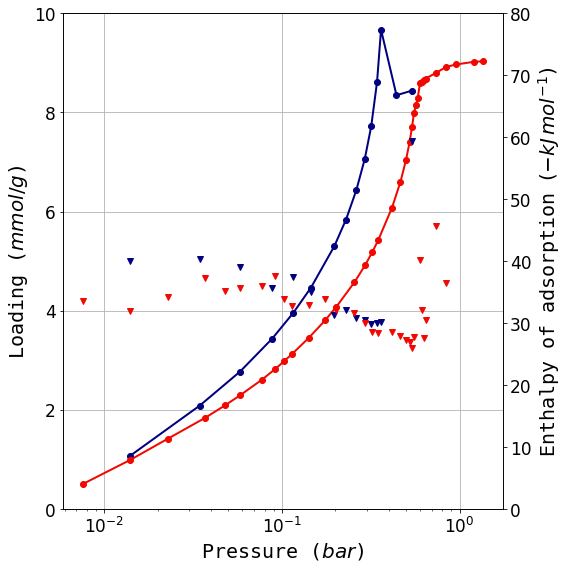
\includegraphics[width=\linewidth]{rtc/dut-sat-log}%
        \caption{}\label{dut:fgr:dut-sat-log}
    \end{subfigure}%
    \begin{subfigure}{0.33\linewidth}
        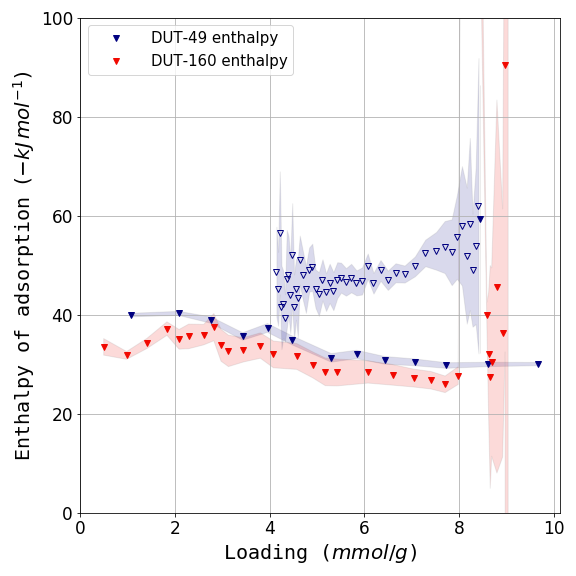
\includegraphics[width=\linewidth]{rtc/dut-sat-enth}%
        \caption{}\label{dut:fgr:dut-sat-enth}
    \end{subfigure}%
    \caption{(a) Experimental adsorption isotherms for DUT-49 and 
    DUT-160. Enthalpy points are omitted for clarity. 
    (b) A logarithmic plot of isotherms and enthalpy curves,
    to highlight the low pressure region. 
    (c) Differential enthalpy of adsorption as a function of loading
    together with the uncertainty range for each measurement.}%
    \label{dut:fgr:dut-sat}
\end{figure}

From its isotherm slope change in \autoref{dut:fgr:dut-sat-reg},
DUT-160 can be seen to undergo a sharp transition at 
\(0.2~p/p_0\), without NGA. The isotherm is very similar to the one
measured on DUT-50, whose linker is comparable in length, pointing to 
a similar buckling behaviour. The lack of NGA is likely due to 
a lower energetic barrier between the \textbf{op} and \textbf{cp}
state. The enthalpy curve of both DUT-160 and 50 has the same 
shape, although the differential enthalpy of adsorption on 
DUT-160 is lower across the entire loading range, a consequence of the
larger uncertainty in the measurement.

\subsubsection{Overview of NGA tuning through different methods}

This extensive study of different DUT-49 derivatives demonstrates the 
large range of options available for tuning structural 
transitions in the prototypical NGA material. Both linker 
shortening and functionalisation lead to increased framework
stiffness, in an analogue fashion to increasing the 
structural integrity of a pillar. This approach might allow 
for the design of materials which would only undergo an 
\textbf{op/co} transition with desired adsorbates and
temperature ranges, or limit structural collapse to mechanical 
pressure. The porosity limit at which net interpenetration begins
to occur is found around the length of the DUT-151 linker, 
or 4 phenyl rings between terminal moieties, a process which does 
not completely suppress flexibility. More importantly, more 
fundamental changes to the type of flexibility, such as 
a continuous ``breathing'' phase transition, or light-induced
switchability might be induced with careful choice of linker,
as seen in DUT-171 and suspected in DUT-161, respectively.